\documentclass[11pt]{article}
\usepackage[paperwidth=13.33in,paperheight=7.5in,top=0.3in,bottom=0.25in,left=0.55in,right=0.55in]{geometry}
\usepackage{amsmath,amssymb}
\usepackage{tikz}
\usepackage{xcolor}
\usepackage{array}
\usepackage{colortbl}
\usepackage{helvet}
\pagestyle{empty}
\setlength{\parindent}{0pt}
\definecolor{lab}{gray}{0.38}
\definecolor{cy}{RGB}{30,145,185}
\definecolor{og}{RGB}{215,120,20}
\definecolor{dens}{RGB}{205,224,242}
\definecolor{holec}{RGB}{248,212,168}
\definecolor{stepn}{RGB}{60,60,60}

% the two tunable parameters: ONE colour each, EVERY occurrence, no exceptions.
\newcommand{\mm}{{\color{cy}m}}
\newcommand{\rr}{{\color{og}\rho}}
\newcommand{\cir}[2]{\tikz[baseline=(n.base)]{\node[draw=#1,line width=0.9pt,circle,inner sep=1.3pt](n){$#2$};}}
\newcommand{\stepttl}[2]{{\sffamily\color{stepn}\textbf{#1}\ \ #2}}
\newcommand{\gloss}[1]{{\sffamily\scriptsize\color{lab}#1}}

\begin{document}
\vspace*{\fill}

{\sffamily\fontsize{24}{28}\selectfont Simulated Data \;--- sparsity (holes) in pseudotime}

\vspace{2mm}
{\sffamily\small\color{lab}Replaces the \texttt{latent\_t} row only. Everything downstream
($s_b$, $z_i$, $y_i = z_iW + s_b$, counts) is unchanged.\\
Throughout both slides, {\color{cy}$m$} and {\color{og}$\rho$} are the \emph{same} two numbers
at every occurrence --- there is only one of each.}

\vspace{2.5mm}
\hrule
\vspace{2mm}

\stepttl{1.}{Cut $[0,1]$ into $2\mm+1$ chunks that alternate dense\,/\,hole, starting and ending dense.}

\vspace{1mm}
\begin{minipage}[t]{0.38\textwidth}
\vspace{0pt}
$\displaystyle w_k = \begin{cases} 1 & k \text{ even} \\ \rr & k \text{ odd}\end{cases}$
\qquad
$\displaystyle p_k = \frac{w_k}{Z}$

\vspace{2mm}
$\displaystyle Z \;=\; \sum_{k=0}^{2\mm} w_k
  \;=\; \underbrace{(\mm+1)}_{\text{\# dense}}\!\cdot 1
  \;+\; \underbrace{\mm}_{\text{\# holes}}\!\cdot\,\rr$

\vspace{2mm}
\gloss{$w_k$ = unnormalized weight (line 195).\\
$Z$ = their sum; dividing by it (line 196) makes $\textstyle\sum_k p_k = 1$.\\
$p_k$ = probability one cell lands in chunk $k$ = \texttt{chunk\_prob[k]}.}
\end{minipage}
\hfill
\begin{minipage}[t]{0.58\textwidth}
\vspace{0pt}
\centering
{\sffamily\small the $\mm=3$, $\rr=0.05$ instance}\\[1.5mm]
\renewcommand{\arraystretch}{1.25}
\setlength{\tabcolsep}{4pt}
\begin{tabular}{r|ccccccc}
\sffamily\footnotesize\color{lab} $k$ & $0$ & $1$ & $2$ & $3$ & $4$ & $5$ & $6$ \\
\hline
\sffamily\footnotesize\color{lab} chunk
 & \cellcolor{dens}dense & \cellcolor{holec}hole & \cellcolor{dens}dense & \cellcolor{holec}hole
 & \cellcolor{dens}dense & \cellcolor{holec}hole & \cellcolor{dens}dense \\
\sffamily\footnotesize\color{lab} weight $w_k$
 & $1$ & $\rr$ & $1$ & $\rr$ & $1$ & $\rr$ & $1$ \\
\sffamily\footnotesize\color{lab} $\;\;\;\;\;= $
 & $1$ & $0.05$ & $1$ & $0.05$ & $1$ & $0.05$ & $1$ \\
\hline
\sffamily\footnotesize\color{lab} $p_k = w_k/Z$
 & $.2410$ & $.0120$ & $.2410$ & $.0120$ & $.2410$ & $.0120$ & $.2410$ \\
\end{tabular}

\vspace{1.5mm}
{\small $Z = 4\cdot 1 + 3\cdot 0.05 = 4.15$ \qquad
 ``$k$ even'' and ``dense'' are the \emph{same} condition, not two.}
\end{minipage}

\vspace{2.5mm}
\hrule
\vspace{2mm}

\stepttl{2.}{Draw one cell's pseudotime with two draws: \emph{which} chunk, then \emph{where inside} it.}

\vspace{1mm}
\begin{minipage}[t]{0.52\textwidth}
\vspace{0pt}
$\displaystyle k_i \sim \mathrm{Cat}(p_0,\dots,p_{2\mm})$
\hfill \gloss{which chunk. \texttt{chunk}, line 199}

\vspace{2mm}
$\displaystyle u_i \sim \mathcal{U}(0,1)$
\hfill \gloss{position \emph{within} that chunk --- not pseudotime.}

\hfill \gloss{\texttt{latent\_t\_chunk}, line 201}

\vspace{2mm}
$\displaystyle t_i \;=\; \frac{k_i + u_i}{2\mm+1}$
\hfill \gloss{pseudotime. \texttt{latent\_t}, lines 202--203}

\vspace{2.5mm}
\gloss{$\mathrm{Cat}$ = categorical (weighted die) over $\{0,\dots,2\mm\}$; in code,
\texttt{rng.choice(..., p=chunk\_prob)}.}
\end{minipage}
\hfill
\begin{minipage}[t]{0.44\textwidth}
\vspace{0pt}
{\sffamily\small a real cell (\texttt{cell\_seed=4}, cell 24):}

\vspace{1mm}
$k_i = 3 \;(\text{a hole}), \qquad u_i = 0.9219$

$t_i = \dfrac{3 + 0.9219}{7} = \dfrac{3.9219}{7} = 0.5603$

\vspace{1mm}
\gloss{chunk 3 spans $[0.4286,\,0.5714]$, and $0.5603$ sits $92.19\%$ of
the way across it --- which is what $u_i$ means.}

\vspace{1.5mm}
\gloss{Derivation: lines 202--203 are
\texttt{u*chunk\_size[k] + chunk\_offset[k]}, then \texttt{/total\_size}.
At $h=1$ every \texttt{chunk\_size} is $1$, \texttt{chunk\_offset[k]} $=k$,
\texttt{total\_size} $=2\mm{+}1$. Substitute. Not a standard formula --- just those two lines.}
\end{minipage}

\vspace*{\fill}
\newpage
\vspace*{\fill}

{\sffamily\fontsize{24}{28}\selectfont Sparsity (holes) \;--- the equivalent density}

\vspace{2mm}
{\sffamily\small\color{lab}Marginalizing $k_i$ out of slide 1 gives a two-level step density
on $[0,1]$. Same distribution, one line.\\
Same {\color{cy}$m$} and {\color{og}$\rho$} as slide 1.}

\vspace{3mm}
\hrule
\vspace{5mm}

\begin{minipage}[t]{0.42\textwidth}
\vspace{0pt}
$\displaystyle t_i \sim f_T, \qquad
 f_T(t) = \frac{2\mm+1}{Z}\begin{cases} 1 & t \notin \mathcal{H} \\ \rr & t \in \mathcal{H}\end{cases}$

\vspace{3mm}
$\displaystyle \mathcal{H} = \bigcup_{j=1}^{\mm}
   \left[\frac{2j-1}{2\mm+1},\ \frac{2j}{2\mm+1}\right)$

\vspace{1mm}
\gloss{$j$ indexes the holes, $1$ to $\mm$. It is a counter, not a parameter.}

\vspace{3mm}
{\footnotesize
\cir{cy}{m} $=\texttt{n\_holes}$: how many low steps. \quad
\cir{og}{\rho} $=\texttt{hole\_density}$: how \emph{low} they are.\\
$h=\texttt{hole\_size}$: how \emph{wide} they are. $h=1$ always, so all
steps are equally wide and $h$ drops out above.\\[1mm]
General $h$: $S=(\mm{+}1)+\mm h$, $Z=(\mm{+}1)+\mm h\rr$,
$f_T=\frac{S}{Z}\rr^{\mathbf{1}[t\in\mathcal H]}$.\\[1mm]
$\mm=0$: one chunk, $Z=1$, $k_i\equiv 0$, so $t_i=u_i\sim\mathcal U(0,1)$ --- the control, unchanged.\\
$\rr=1$: $Z=2\mm{+}1$, so $f_T \equiv 1$ --- also $\mathcal U(0,1)$. A hole at full density is not a hole.}
\end{minipage}
\hfill
\begin{minipage}[t]{0.54\textwidth}
\vspace{0pt}
\centering
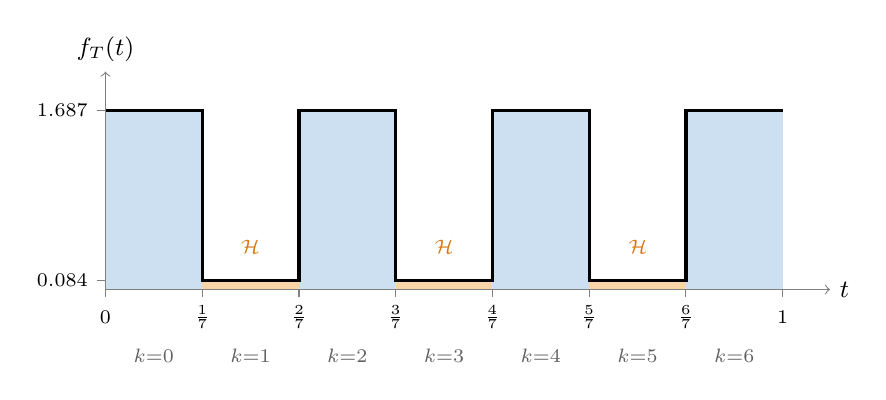
\begin{tikzpicture}[x=8.6cm,y=1.35cm]
  \foreach \a/\b in {0/0.142857, 0.285714/0.428571, 0.571429/0.714286, 0.857143/1.0}
    {\fill[dens] (\a,0) rectangle (\b,1.687);}
  \foreach \a/\b in {0.142857/0.285714, 0.428571/0.571429, 0.714286/0.857143}
    {\fill[holec] (\a,0) rectangle (\b,0.0843);}
  \draw[very thick]
    (0,1.687) -- (0.142857,1.687) -- (0.142857,0.0843) -- (0.285714,0.0843) --
    (0.285714,1.687) -- (0.428571,1.687) -- (0.428571,0.0843) -- (0.571429,0.0843) --
    (0.571429,1.687) -- (0.714286,1.687) -- (0.714286,0.0843) -- (0.857143,0.0843) --
    (0.857143,1.687) -- (1.0,1.687);
  \draw[->,gray] (0,0) -- (1.07,0) node[right,black,font=\small]{$t$};
  \draw[->,gray] (0,0) -- (0,2.05) node[above,black,font=\small]{$f_T(t)$};
  \draw[dashed,gray] (0,1.687) -- (-0.012,1.687) node[left,black,font=\scriptsize]{$1.687$};
  \draw[dashed,gray] (0,0.0843) -- (-0.012,0.0843) node[left,black,font=\scriptsize]{$0.084$};
  \foreach \x in {0,0.142857,0.285714,0.428571,0.571429,0.714286,0.857143,1.0}
    {\draw[gray] (\x,0) -- (\x,-0.07);}
  \node[font=\scriptsize] at (0,-0.26) {$0$};
  \node[font=\scriptsize] at (0.142857,-0.26) {$\frac{1}{7}$};
  \node[font=\scriptsize] at (0.285714,-0.26) {$\frac{2}{7}$};
  \node[font=\scriptsize] at (0.428571,-0.26) {$\frac{3}{7}$};
  \node[font=\scriptsize] at (0.571429,-0.26) {$\frac{4}{7}$};
  \node[font=\scriptsize] at (0.714286,-0.26) {$\frac{5}{7}$};
  \node[font=\scriptsize] at (0.857143,-0.26) {$\frac{6}{7}$};
  \node[font=\scriptsize] at (1.0,-0.26) {$1$};
  \foreach \x/\k in {0.0714/0, 0.2143/1, 0.3571/2, 0.5/3, 0.6429/4, 0.7857/5, 0.9286/6}
    {\node[font=\scriptsize\sffamily,color=lab] at (\x,-0.62) {$k{=}\k$};}
  \node[font=\scriptsize\sffamily,color=og] at (0.214,0.40) {$\mathcal{H}$};
  \node[font=\scriptsize\sffamily,color=og] at (0.5,0.40) {$\mathcal{H}$};
  \node[font=\scriptsize\sffamily,color=og] at (0.786,0.40) {$\mathcal{H}$};
\end{tikzpicture}\\[2mm]
{\footnotesize Gaps in pseudotime \emph{support} --- those cells are never drawn.
Nothing here zeroes $x$; \texttt{adata.X} stays $(2500,200)$.}
\end{minipage}

\vspace*{\fill}
\end{document}
